\documentclass[10pt]{article}
\usepackage[T1]{fontenc}
\usepackage{lmodern,amsmath,amssymb,graphicx,hyperref,array}
\usepackage[margin=.75in]{geometry}
\setlength{\parindent}{0pt}\setlength{\parskip}{6pt}
\begin{document}
\begin{center}
{\Large Compact factors for actual whole crossing charts}\\[4pt]
14 November 2026; 39 authored Lean statements\\
Source \texttt{95f5d5c917a286103a3c74deaa9db431e5196e81}
\end{center}
\textbf{Construction.} The same completed auxiliary orientation polynomial
now has explicit whole-polynomial crossing factors at arbitrary finite
precision, for every retained nonzero source node. The proof constructs the
factors through actual bivariate coefficients and row classes. No basis,
rank witness or favorable coefficient bound is supplied as a premise.
All records are unsigned [pcc:unverified].

\textbf{Actual hypotheses.} Let $L=2^a$, actual ports $x,y<L$, and nonzero
integer $t\in\{-L,\ldots,L-1\}$ with $v_2(t)=i<u\le a$. Matrices explicitly
retain equal-bit-$i$ crossings and zero other entries. Multiplicities $m_j$
are arbitrary naturals. Use the original nonzero negative-pole diagonal $c$,
$w=v_2(c)$, and the same $W_{xy}(T)$, with
\[
 r=x\bmod2^u,\quad h=x\mathbin{\mathrm{div}}2^u,\quad
 \alpha=2^{a+1},\quad P_{xy}(Z)=W_{xy}(t+\alpha Z)/c.
\]
No nonzero local first jet or positive multiplicity is assumed in the general
factor result. The identity origin is unchanged [pcc:unverified].

\textbf{Actual row polynomial.} Put $\delta_r=y-r$,
$e_t=2^u/(t-\delta_r)$, $e_j=2^u/(2^j-\delta_r)$,
$\lambda=\alpha/(t-\delta_r)$, and
\[
 \mathcal D(H,Z)=(1+\lambda Z+e_tH)
      \prod_{j\in M_{ry}}(1+e_jH)^{m_j},\qquad
 N(Z)=(1+\lambda Z)P_{ry}(Z).
\]
Actual masks and denominators give even $e_t,e_j,\lambda$. Substituting the
actual integer $h$ gives exactly the previous component's actual denominator
$D(Z)$, with $DP_{xy}=N$ and $D-1$ of content one. These bridges are derived
from the original completed polynomials, not assumed [pcc:unverified].

Define
\[
 \mathcal A(H,Z)=N(Z)\sum_{n<k}(1-\mathcal D(H,Z))^n.
\]
Its coefficient of $H^b$ has polynomial content at least $b$ in $Z$.
The proof derives this using actual even slopes and explicit polynomial
closure. At integer $h$, removing all terms $b\ge k$ has content-$k$ error.
The remaining finite sum approximates every coefficient of $P_{xy}$ at
precision $k$ [pcc:unverified].

\newpage
\begin{center}{\Large Literal factors and actual weighted residual}\end{center}
For each representative $r\in\mathrm{Fin}(2^u)$ and $b\in\mathrm{Fin}(k)$,
define polynomial matrices
\[
 U_{x,(r,b)}=\begin{cases}2^b h^b&r=x\bmod2^u,\\0&\text{otherwise},\end{cases}
 \qquad
 V_{(r,b),y}=2^{-b}[H^b]\mathcal A_{ry}(H,Z),
\]
where the right factor is explicitly zero if $r,y$ do not cross at bit $i$.
The left scalar is viewed as a constant polynomial in $Z$.
The representative construction depends only on the row class, so finite
matrix multiplication selects its actual truncated row polynomial
[pcc:unverified].

All right factors are integral in every $Z$ coefficient because
$[H^b]\mathcal A$ has content at least $b$. The left has content at least $b$.
For the normalized crossing polynomial matrix $P^{\rm cross}$,
\[
 \operatorname{Content}_k(P^{\rm cross}_{xy}-(UV)_{xy}).
\]
The factors are constructed for the whole polynomial, including higher
chart coefficients, rather than just its first jet [pcc:unverified].

Scale the left factor by the same actual $c$ and call it $\widehat U$.
For the actual unnormalized crossing chart matrix $W^{\rm cross}$,
\[
 \operatorname{Content}_{w+b}(\widehat U_{x,(r,b)}),\qquad
 \operatorname{Content}_0(V_{(r,b),y}),\qquad
 \operatorname{Content}_{w+k}
     (W^{\rm cross}_{xy}-(\widehat U V)_{xy}).
\]
Scaled-left integrality follows when $w\ge0$. Exact inner-label cardinality
is $2^u k$, including the empty $k=0$ case. Every label is charged
[pcc:unverified].

\textbf{Scope at anchor zeros.} The derivation does not cancel a local first
jet. Positive anchors where that jet vanishes remain included. Previous
first-jet zero controls concern first jets only. This component makes no
low-rank statement for all unmasked $W$ or for its identity origin
[pcc:unverified].

\textbf{What the count does not price.} The component gives whole-polynomial
content and explicit factors. It does not yet bound each right factor's
necessary degree at precision $k$, coefficient bit sizes, entry construction,
creation precision or total running time. Those are the next proof tasks.

\newpage
\begin{center}{\Large Dependency map and original mode costs}\end{center}
\begin{center}
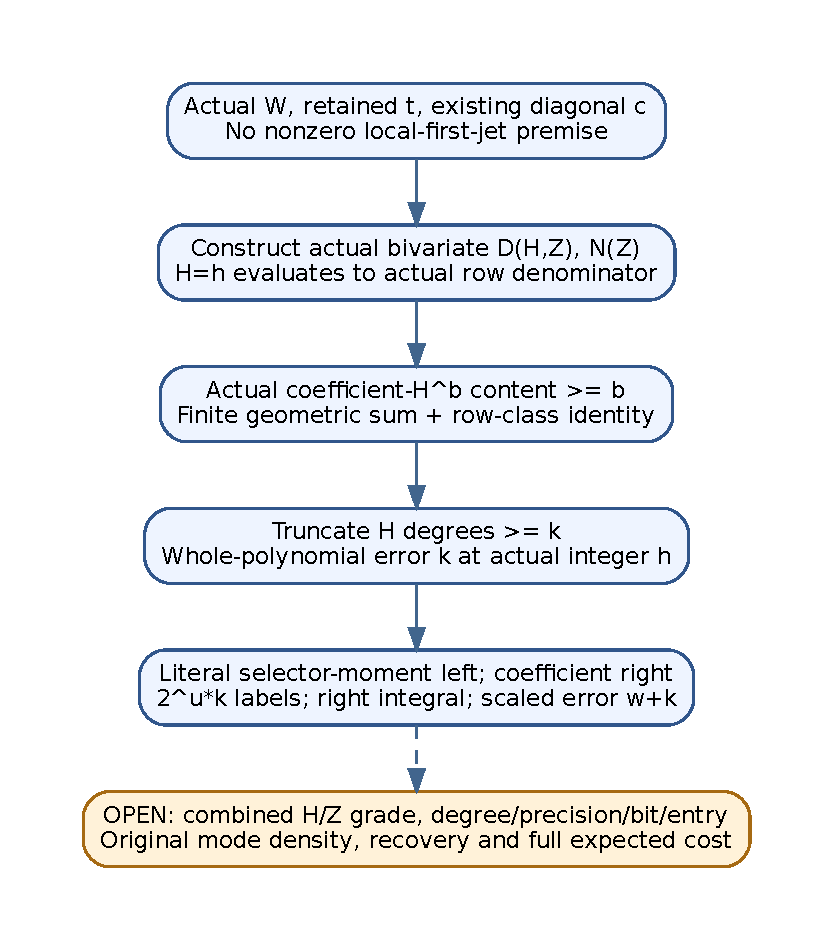
\includegraphics[width=.96\linewidth,height=4.5in,keepaspectratio]{dependencies.pdf}
\end{center}
The reviewed original interface allows at most $6M/D_i$ modes per weight,
$D_i=L/2^i$, and at most $3M/L$ packets. The present construction retains
$2^u$ row classes at every moment index; that can exceed the old $2^{i+1}$
tile inventory. A factor count alone does not establish a runtime gain
[pcc:unverified].

\textbf{Next discriminating proof.} Establish combined $H/Z$ coefficient
grading, then truncate right $Z$ degree at the requested residual while
retaining the actual matrix error. Price all coefficient construction,
entry and bit operations, degree, precision, recovery and recursion against
the original weighted mode interface. Actual elliptic relation, efficient
public finder, field and scalar extraction, retries and full expected bit
cost remain explicit obligations. No sub-exponential runtime or algorithm
conclusion follows from this component.

\newpage
\begin{center}{\Large Source bindings, checks and preservation}\end{center}
The isolated project builds 39 authored statements without warnings.
The pinned shared audit covers39 declarations,0 extra trusted axioms,
exit0. Import-inclusive fresh replay is running, not passed. Five central
printed dependencies contain only \texttt{propext}, \texttt{Classical.choice},
\texttt{Quot.sound}. All records are unsigned [pcc:unverified].

\begin{center}\small
\begin{tabular}{p{.63\linewidth}p{.26\linewidth}}
\texttt{denom\_rows\_eval}&PCC-20261114-4f155f\\
\texttt{actual\_low\_rows\_precision}&PCC-20261114-e87981\\
\texttt{poly\_right\_integral}&PCC-20261114-8af989\\
\texttt{actual\_compact\_poly\_precision}&PCC-20261114-ce6456\\
\texttt{actual\_compact\_weighted\_profile}&PCC-20261114-6a7512
\end{tabular}
\end{center}
Exact statements govern every hypothesis. Source/configuration pins, full
statement bindings and the prospective contract are in
\begin{center}\small
\path{../evidence/source-freeze.json}\\
\path{../evidence/claim-pins.json}\\
\path{../PROTOCOL.md}.
\end{center}
Gate data is PCC-20261114-92f882. Local accepted008 data is
PCC-20261114-91d645; it alone is not independent
gate/replay coverage [pcc:unverified].

\textbf{Pinned environment.} Lean4.35.0, CryptoLean and Mathlib revisions:
\begin{center}\small
\texttt{148f5dc389b341401e06d76abe7783c4ccf42f2e}\\
\texttt{cfc55fc58714a59dc06e6e79edc6d1d95140d3c2}.
\end{center}
The source is byte-identical accepted008. All eight local drafts and raw
build logs/exits remain in the parent bivariate evidence directory.
Failed attempts include missing Content/Jet namespaces, an ambiguous slope,
and a misidentified valuation-lemma namespace. Failed elaboration diagnostics
including \texttt{sorryAx} remain raw evidence; accepted008 contains no such
dependency. No linter was disabled or favorable hypothesis added.

\textbf{Sources checked.} KB unavailable as journaled. Read exact Higher,
Node, Moment and Content coefficient, evaluation, row-class and truncation
APIs; pinned Mathlib polynomial and power-series truncation APIs; primary
D.4.3--7 and prior contraction cost/precision reviews. Standard bivariate
polynomials and geometric sums are reused, with no novelty, priority,
fastest-method or measured timing claim.

No native crypto, attack, F4/msolve, timing, scaling, paid or cloud experiment
ran. The original norm fixture remains unlaunched under its unchanged
transport blocker. Canonical IC graphs/leaderboards have no new measured
result; this diagram describes proof dependencies.

Higher83 and Node90 checkpoint artifacts and all earlier parent sources,
reports, claims and raw outputs remain exact. Protected concurrent PCC
histories still need legitimate canonical-maintainer reconciliation;
auto-merge stays off. No choose-side, rechain, claim rewrite, signature,
trust change, prefix waiver, force push or merge is attempted.
\end{document}
